\documentclass[11pt]{article}
\usepackage{amsmath}
\usepackage{listings}
\usepackage{graphicx}


\newcommand{\numpy}{{\tt numpy}}    % tt font for numpy

\topmargin -.5in
\textheight 9in
\oddsidemargin -.25in
\evensidemargin -.25in
\textwidth 7in

\begin{document}

% ========== Edit your name here
\author{Yao Xiao}
\title{Homework 9: Digital Signature: Due by 12:00AM Thursday, 5 December 2019}
\maketitle

\medskip

% ========== Begin answering questions here
\begin{enumerate}

\item
Answer to question 1:

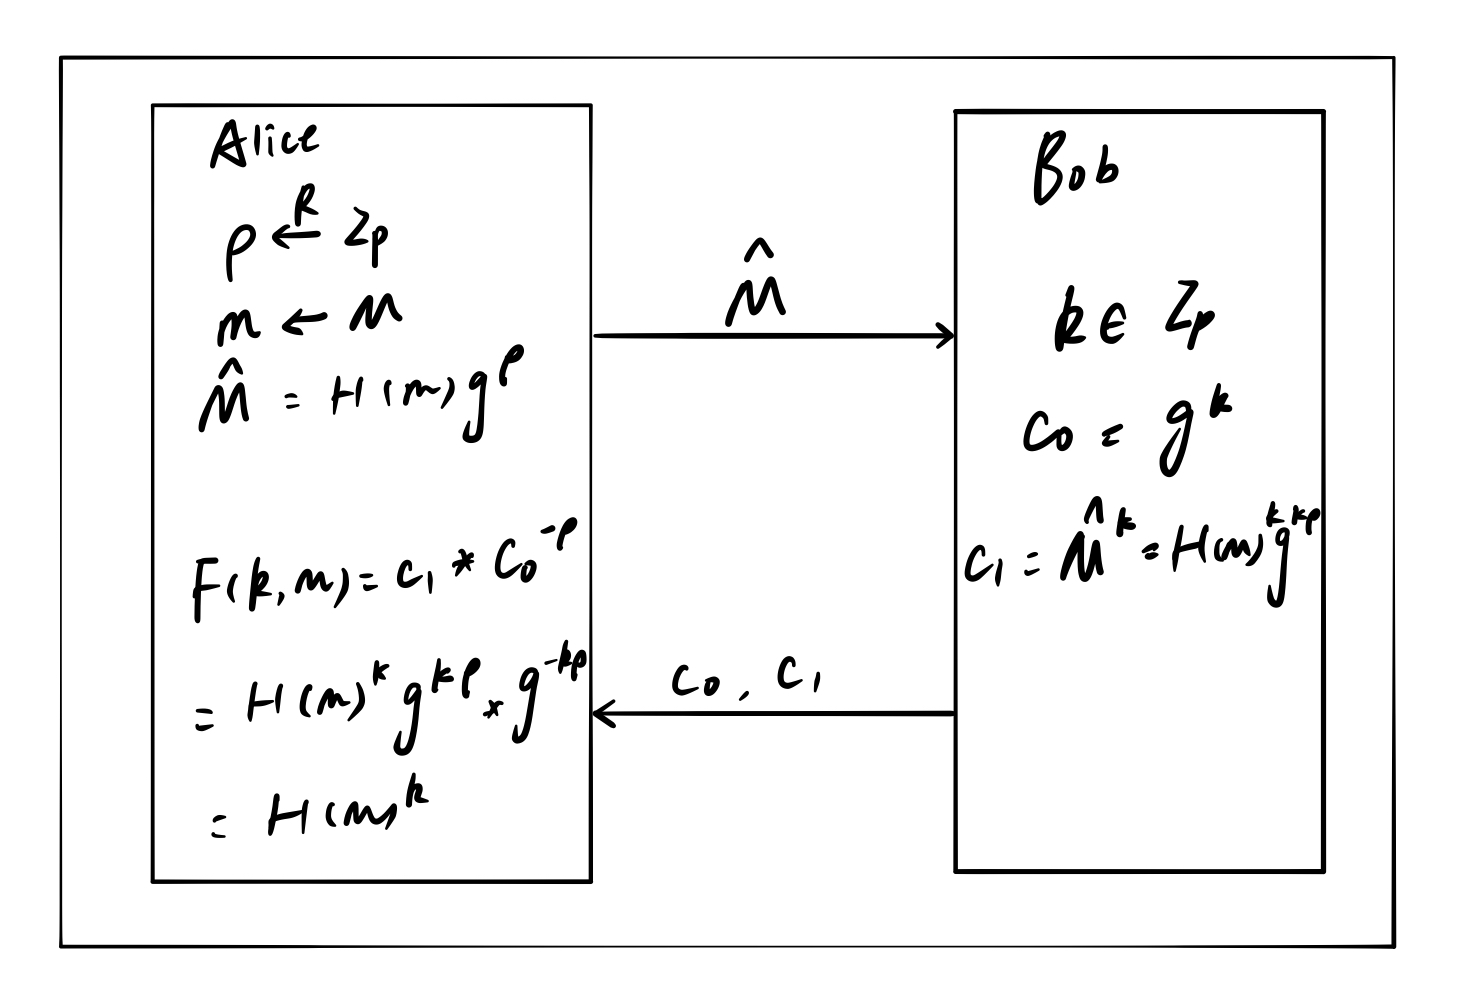
\includegraphics[scale=0.3]{S1.jpeg}

Finally, Alice compute $u = H(m)^k \cdot g^{p \cdot k} \cdot g^{-p \cdot k} = H(m)^k$, and get $F(k,m) = H(m)^k$


\item
Answer to question 2:

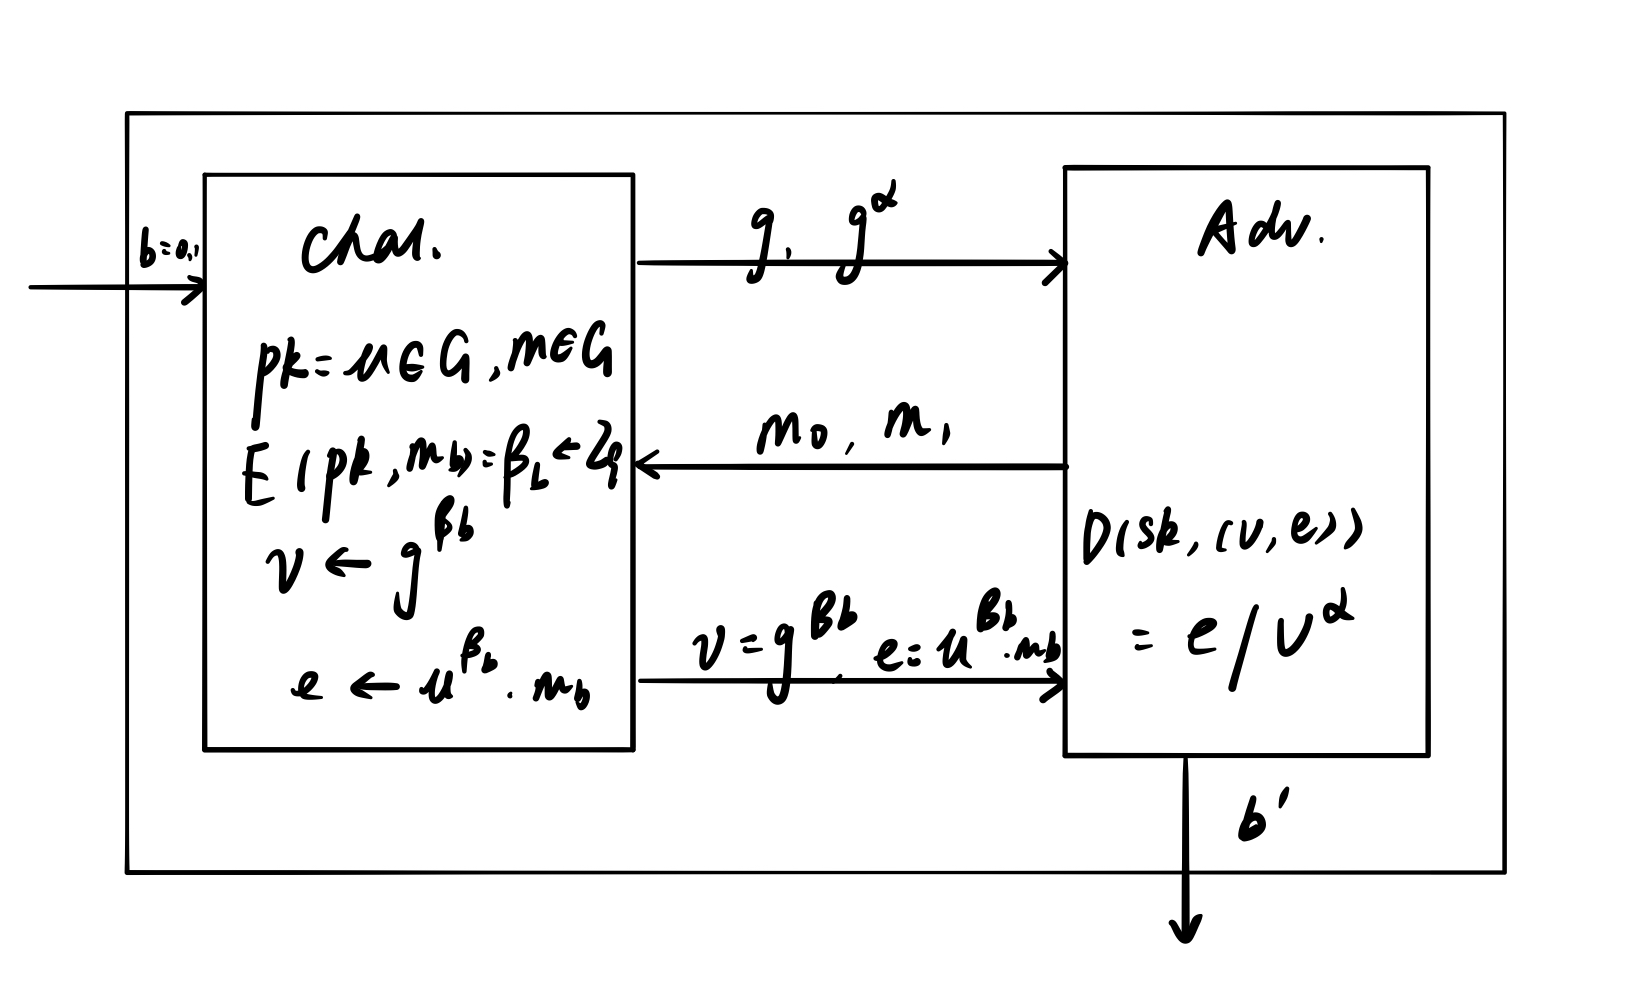
\includegraphics[scale=0.3]{S2.jpeg}

\begin{enumerate}
    \item In DHH assumption, adv. can't distinguish $g^{\alpha \cdot \beta}$ and $g^{c}$, if chal. encrypt the $m_0$ and send (v,e), adv. can not know $v^{\alpha}$ whether is $g^{\alpha \cdot \beta_0}$ or $g^{\alpha \cdot \beta_1}$, in the end it can't be distinguished from $(g^{\alpha},g^{\beta},g^{\alpha \cdot \beta})$ and $(g^{\alpha},g^{\beta},g^{c}).$\\
          So $Adv_SS[A,E]$ = $|Pr\left[W_0\right] - Pr\left[W_1\right]|$ is negligible, the $E_{MEG}$ is semantically secure.
    \item If DHH assumption does note hold in G, adv. can distinguish $g^{\alpha \cdot \beta}$ and $g^{c}$, if chal. encrypt hte $m_0$ and send (v,e), adv. can know $v^{\alpha}$ whether is $g^{\alpha \cdot \beta_0}$ or $g^{\alpha \cdot \beta_1}$, in the end it can't be distinguished from $(g^{\alpha},g^{\beta},g^{\alpha \cdot \beta})$ and $(g^{\alpha},g^{\beta},g^{c}).$ or not.\\
          So $Adv_SS[A,E]$ = $|Pr\left[W_0\right] - Pr\left[W_1\right]|$ = 1, the $E_{MEG}$ is not semantic secure.
    \item when adv. compute $m_1 \cdot m_2 = D(sk,(v_1,e_1)) \cdot D(sk,(v_2,e_2)) = (e_1/v^{\alpha}_1) \cdot (e_2 / v^{\alpha}_{1})$\\
          $\frac{u^{\gamma} \cdot (m_1 \cdot m_2h)}{g^{\alpha \gamma}} = (u^{\gamma} \cdot (m_1 \cdot m_2) / g^{\alpha \gamma}) = m_1 \cdot m_2$\\
          when chal. encrypt $m_1 \cdot m_2$ and $E(pk,(m_1 \cdot m_2)) = c$\\
          $m_1 \cdot m_2 = \frac{u^{c} \cdot (m_1 \cdot m_2)}{g^{\alpha^{c}}} = (u^{c} \cdot (m_1 \cdot m_2/ g^{\alpha^{c}}) = (u^{\gamma} \cdot (m_1 \cdot m_2) / g^{\alpha^{\gamma}})$\\
          $c = \gamma = \beta_1 + \beta_2$\\
          $E(pk,(m_1 \cdot m_2)) = c = \beta_1 +\beta_2$\\
          So it is a multiplicative homomorphism.
\end{enumerate}


\item
Answer to question 3:

\begin{enumerate}
    \item 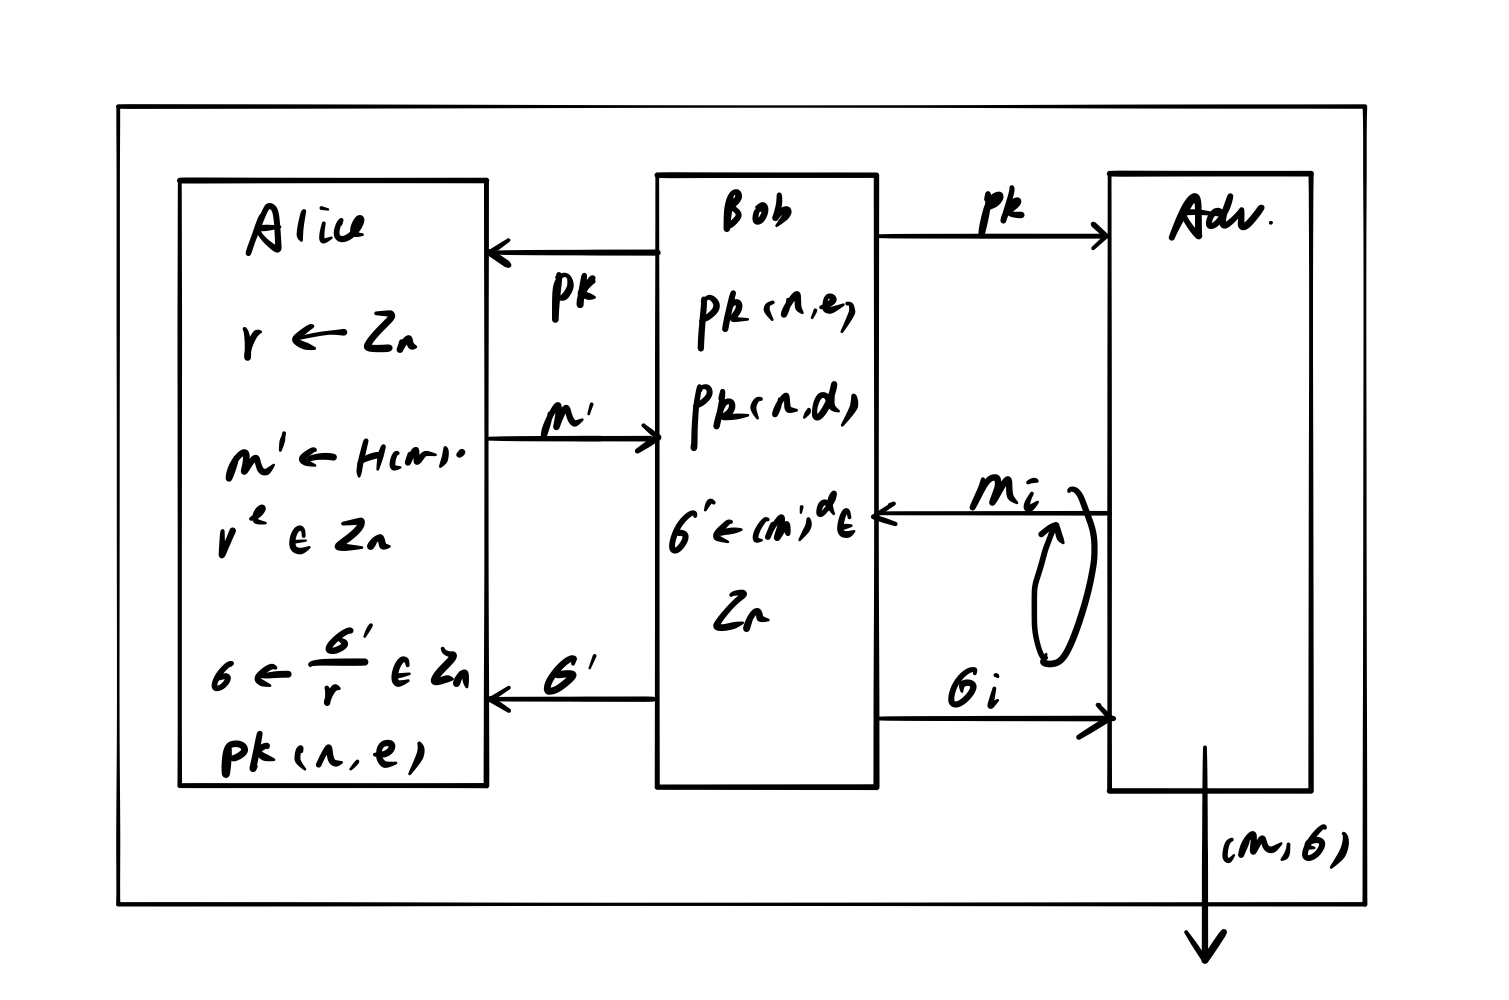
\includegraphics[scale=0.3]{S3_1.jpeg}
    \item 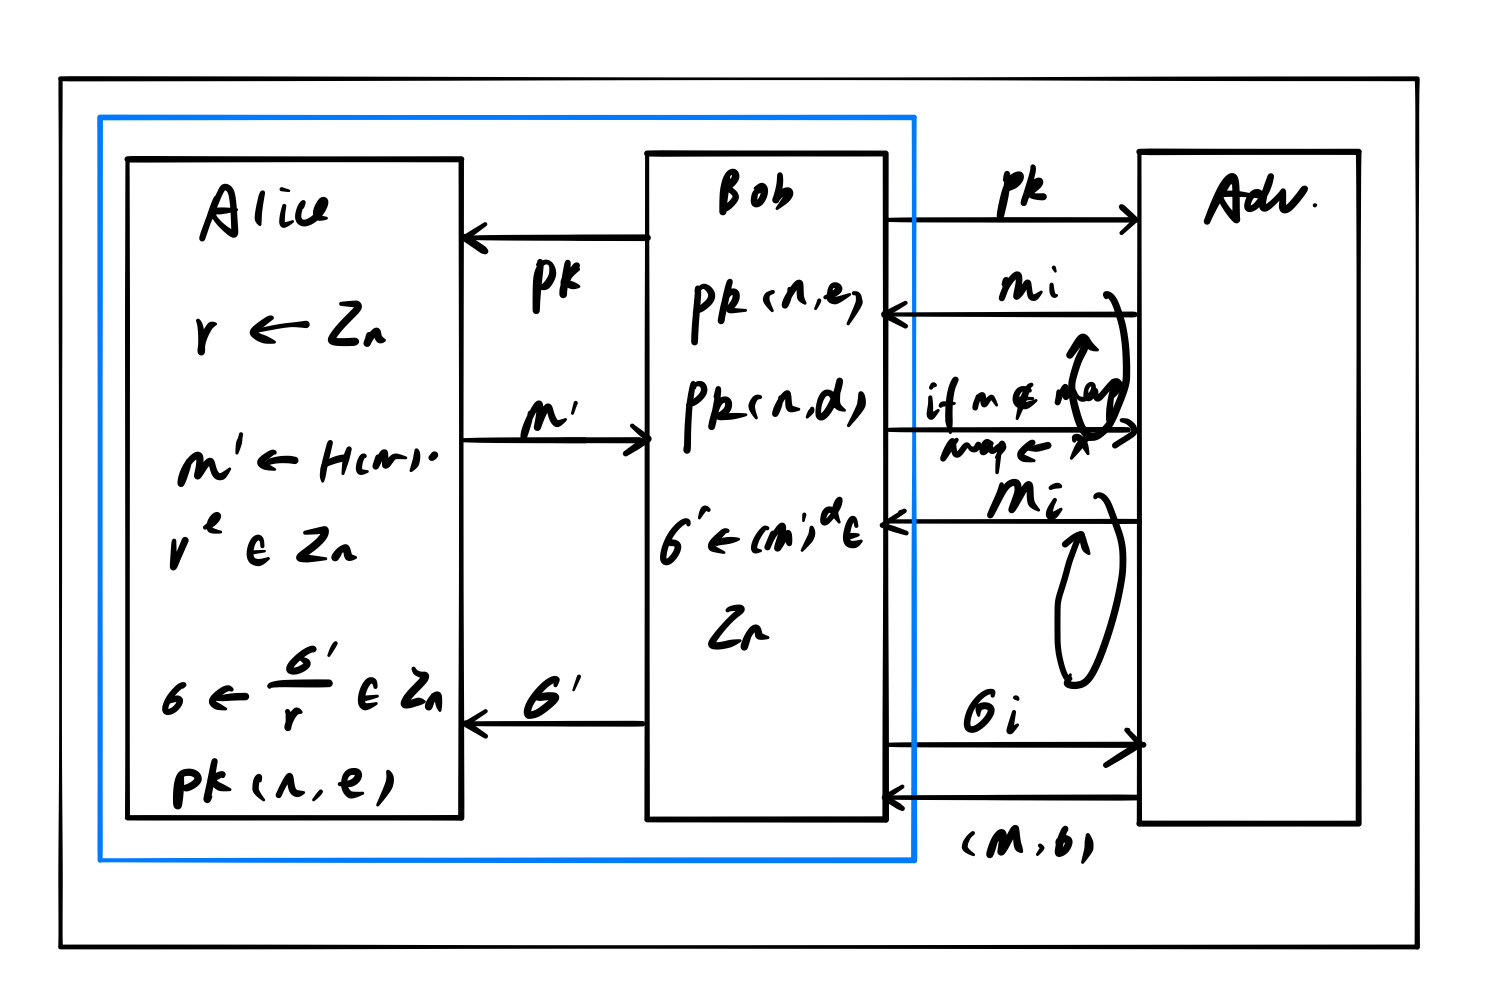
\includegraphics[scale=0.3]{S3_2.jpeg}
\end{enumerate}

\item
Answer to question 4:

\begin{enumerate}
    \item D = $g^{a}, h^{b}$, $e(g^{a},g^{b}) \in G^{4}$ is a DH-tuple if $\alpha\beta = \gamma$. Then $\alpha\beta = \gamma \Leftrightarrow e(g^{\alpha},g^{\beta}) = e(g,g^{\gamma})$\\
          In DDH assumption, when you get $g^{a}, h^{b}$, $e(g^{a},g^{b}) == e(g,h)^{ab}$ can be computed. Once knowing $e(g,h)^{ab}$, it can see which group is $(g^{a},h^{b},e(g,h)^{ab})$.
    \item 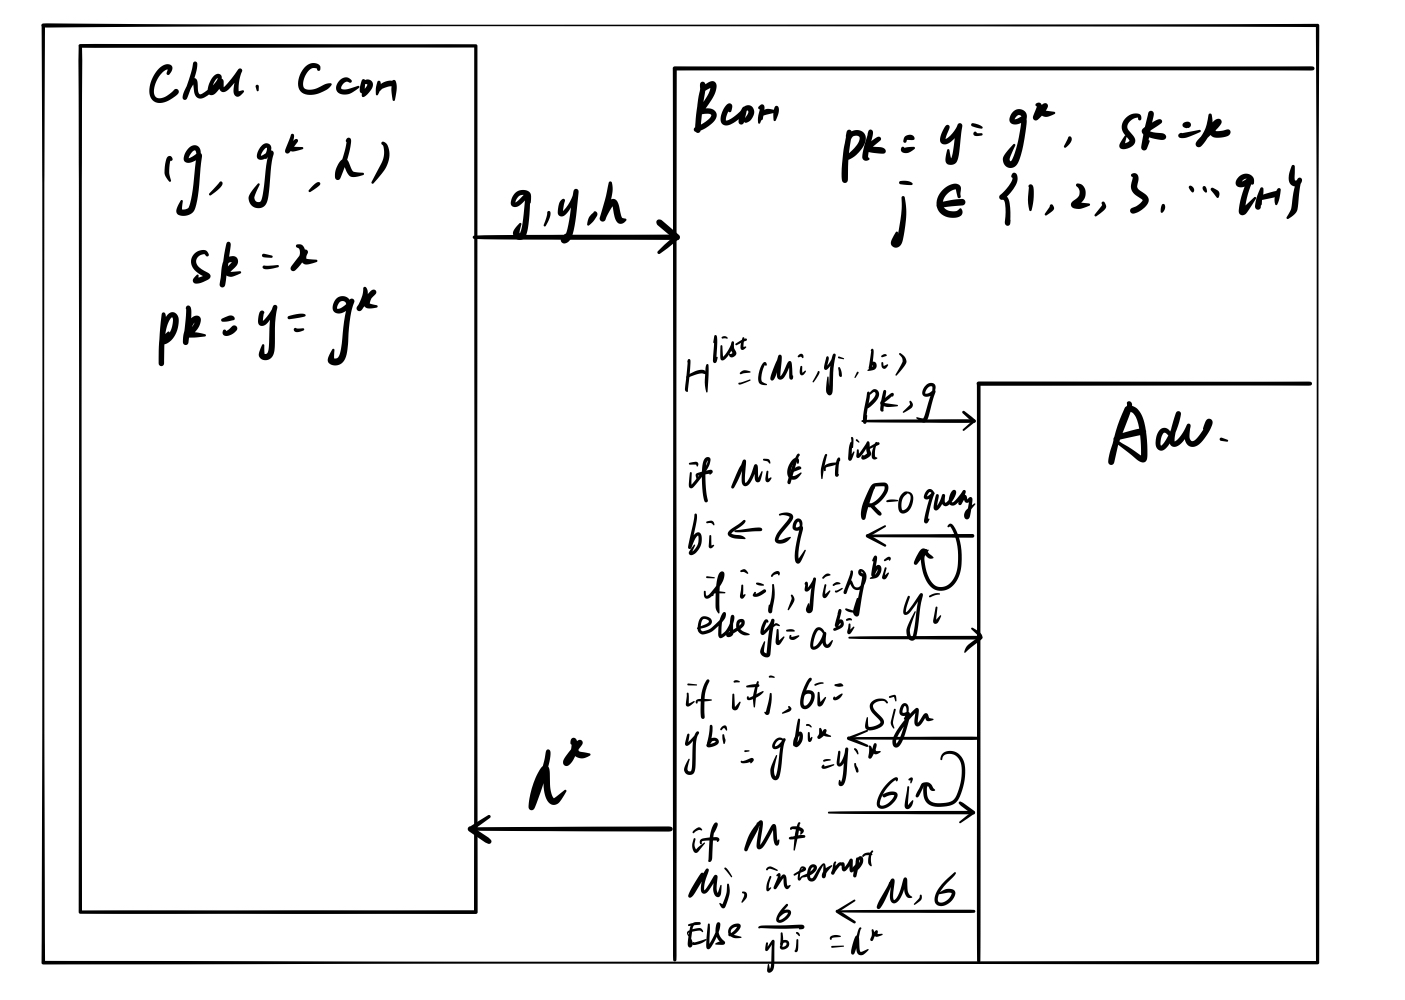
\includegraphics[scale=0.3]{S4.jpeg}\\
          $\sigma = y^{x}_j = (hg^{b_j})^{x} = h^{x}g^{b_jx} = h^{x}(g^{x})^{b_j} = h^{x}y^{b_j}$
\end{enumerate}


\end{enumerate}

\end{document}
\grid
\grid